\documentclass[a4paper,12pt]{ncc}
 \usepackage[warn]{mathtext}
 \usepackage[T2A]{fontenc}
 \usepackage[utf8]{inputenc}
 \usepackage[english,russian]{babel}
 \usepackage{indentfirst}
 \title{Глобальное потепление и его последствия}
 \author{Геворкян Виктория, ФиКЛ}
\usepackage{graphicx}
\graphicspath{{pictures/}}
\DeclareGraphicsExtensions{.pdf,.png,.jpg}
\usepackage{multirow}%для таблицы
 \begin{document}
 \maketitle{}
 \tableofcontents{}
 \section{Что такое глобальное потепление?}
 \label{sec:section}
 Глобальное потепление — это медленное и постепенное увеличение средней температуры на нашей планете, которое как раз наблюдается в настоящее время. Глобально потепление — это факт, спорить с которым бессмысленно, и именно поэтому необходимо трезво и объективно подойти к его осмыслению.
\section{Причины глобального потепления}
\label{sec:section}
 По научным данным, глобальное потепление может быть вызвано множеством факторов:
\begin{itemize}

\item извержения вулканов;
\item поведение Мирового океана (тайфуны, ураганы и т.д.);
\item солнечная активность;
\item магнитное поле Земли;
\item деятельность человека. Так называемый антропогенный фактор. Идея поддерживается большинством ученых, общественных организаций и СМИ, что вовсе не означает ее непоколебимую истинность.
\end{itemize}

Скорее всего, окажется, что каждая из этих составляющих вносит свой вклад в глобальное потепление.
 \section{Какие факты доказывают глобальное потепление?}
 \label{sec:section}
 
 \subsection{Рост температур}
 \label{sec:subsection}
За температурой документально наблюдают около 150 лет. Принято считать, что она поднялась где-то на $0,6^\circ$ С за прошедшее столетие, хотя до сих пор четкой методики определения этого параметра не существует, так же нет уверенности в адекватности данных столетней давности. Поговаривают, что потепление резко с 1976 года, начала бурной индустриальной деятельности человека и максимального ускорения достигло во второй половине 90-х годов. Но и тут есть расхождения между наземными и спутниковыми наблюдениями.

 \subsection{Поднятие уровня мирового океана}
 \label{sec:subsection}
В результате потепления и таяния ледников в Арктике, Антарктиде и Гренландии, уровень воды на планете поднялся на 10-20 см, возможно больше.\cite[Волкова]{volkova-2006}


 \subsection{Таяние ледников}
 \label{sec:subsection}
Ну что тут скажешь, глобальное потепление действительно является причиной таяния ледников, и лучше слов это подтвердят фотографии.

\begin{figure}[h]
\center{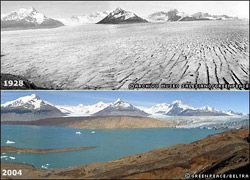
\includegraphics[scale=0.9]{1.jpg}}
\caption{Ледник Упсала в Патагонии (Аргентина) был одним из самых больших ледников Южной Америки, но теперь исчезает на 200 метров в год.}
\label{fig:image}
\end{figure}

\begin{figure}[h]
\center{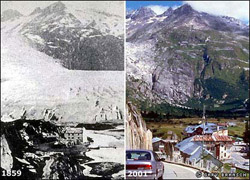
\includegraphics[scale=0.9]{2.jpg}}
\caption{Ледник Роун, Валаис, Швейцария поднялся вверх на 450 метров.}
\label{fig:image}
\end{figure}

\begin{figure}[h]
\begin{minipage}[h]{0.49\linewidth}
\center{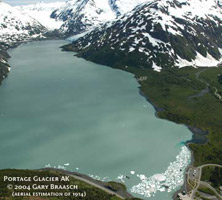
\includegraphics[width=0.5\linewidth]{3} \\ а)}
\end{minipage}
\hfill
\begin{minipage}[h]{0.49\linewidth}
\center{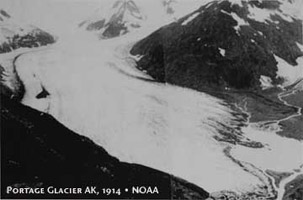
\includegraphics[width=0.5\linewidth]{3-2} \\ б)}
\end{minipage}
\caption{Ледник портадж в Аляске.}
\label{ris:image1}
\end{figure}

\begin{figure}[h]
\begin{minipage}[h]{0.49\linewidth}
\center{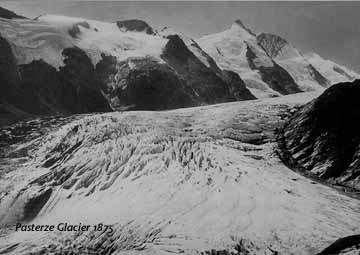
\includegraphics[width=0.5\linewidth]{4} \\ а)}
\end{minipage}
\hfill
\begin{minipage}[h]{0.49\linewidth}
\center{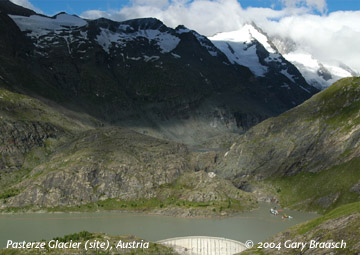
\includegraphics[width=0.5\linewidth]{4-2} \\ б)}
\end{minipage}
\caption{1875 photo courtesy H. Slupetzky/University of Salzburg Pasterze.}
\label{ris:image1}
\end{figure}


\subsubsection[Взаимосвязь глобального потепления и мировых катаклизмов]{Взаимосвязь глобального потепления и мировых катаклизмов}
\label{sec:subsubsection}

\begin{figure}[!h]
\center{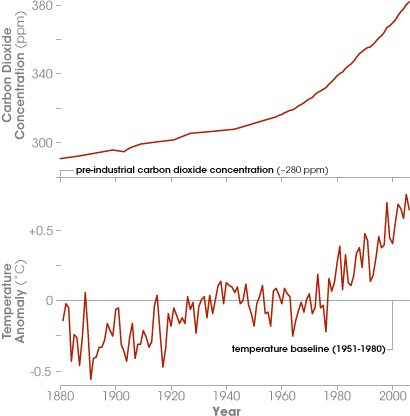
\includegraphics[scale=0.465, angle=180]{5}}
\end{figure}

\subsubsection[Что может влиять на климат?]{Что может влиять на климат?}
\label{sec:subsubsection}
 
 
 \begin{enumerate}
\item \textbf{Вариации радиуса и вытянутости земной орбиты.} Расстояние от Земли до Солнца изменяется не только на масштабах времен порядка 100 миллионов лет, но и с периодом около 20 тысяч лет. При этом уровень летней инсоляции полушарий регулярно варьируется почти на 10\% из-за удаления от Солнца. 
\item \textbf{Колебания наклона земной оси.} Наклон земной оси к плоскости орбиты составляет $23,5^\circ$ и испытывает колебания величиной $1^\circ$ за десятки и сотни тысяч лет. Эти изменения влияют на температурный контраст между высокими и низкими широтами. 
\item \textbf{Флуктуации интенсивности космических лучей.} Космические лучи ионизируют атомы в атмосфере Земли. Ионы служат центрами конденсации водяного пара и способствуют образованию облаков, что повышает альбедо Земли. Интенсивность космических лучей меняется при движении Солнечной системы по Галактике. 
\item \textbf{Изменение светимости Солнца.} Сейчас количество энергии, поступающей от Солнца, колеблется очень незначительно (примерно на 0,1\%). Между тем нельзя исключить более значительных колебаний на длительных отрезках времени. 
\item \textbf{Переполюсовка земного магнитного поля.} Характерный масштаб — порядка четверти миллиона лет. Правда, последняя переполюсовка произошла 780 тысяч лет назад. В момент смены полярности атмосфера в меньшей мере защищена от действия солнечного ветра и космических лучей. 
\item \textbf{Парниковые газы в атмосфере.} Удерживают инфракрасное излучение Земли, препятствуя его уходу в космос. 
\item \textbf{Изменения ландшафтов.} От характера земной поверхности и растительности на ней зависит количество рассеиваемого излучения и в конечном счете альбедо Земли. В частности, существенное влияние на ландшафт оказывают сельское хозяйство и урбанизация. 
\item \textbf{Падения астероидов, крупные вулканические извержения, ядерные взрывы на поверхности Земли.} Выброс аэрозолей в стратосферу уменьшает количество солнечной энергии, поступающей на Землю, а пыль в тропосфере увеличивает облачность — так называемый эффект «ядерной зимы». Продолжительность — от нескольких месяцев до десятков лет.
\end{enumerate}

 \section*{Методы предсказывания глобального потепления} %Раздел, отсутствующий в содержании
 
 Глобальное потепление и его развитие предсказывают, в основном, с помощью компьютерных моделей, на основе собранных данных о температуре, концентрации углекислого газа и много чего еще. Разумеется, точность подобных прогнозов оставляет желать лучшего и, как правило, не превышает 50\%, причем, чем дальше замахиваются ученые, тем меньше становится вероятность сбывания предсказания.

Так же для получения данных используют сверхглубокое бурение ледников, иногда пробы берутся с глубины до 3000 метров. Этот древний лед хранит в себе информацию о температуре, солнечной активности, интенсивности магнитного поля Земли того времени. Информация используется для сравнения с показателями настоящего времени.\cite[Елдышев]{eldyshev-2009}.


 \section{Площади основных типов растительного покрова территории России при глобальном потеплении и динамика их изменения}
 \label{sec:section}
 
\begin{table}[!h]
\centering
\caption{Площади основных типов растительного покрова территории России при глобальном потеплении и динамика их изменения}
\label{my-label}
\begin{tabular}{|l|c|c|c|}
\hline
\multirow{2}{*}{\begin{tabular}[c]{@{}l@{}}Основные типы \\ растительного покрова\end{tabular}} & \multicolumn{3}{c|}{Площади растительных зон (тыс. км-)}                                                                                                                                                         \\ \cline{2-4} 
                                                                                                & \begin{tabular}[c]{@{}c@{}}Современный \\ климат\end{tabular} & \begin{tabular}[c]{@{}c@{}}При глобальном\\  потеплении\end{tabular} & \begin{tabular}[c]{@{}c@{}}Величина изменения\\  площади зон\end{tabular} \\ \hline
Тундра                                                                                          & 5355                                                          & 1584                                                                 & -3771                                                                     \\ \hline
Тайга                                                                                           & 8898                                                          & 6384                                                                 & -2514                                                                     \\ \hline
Лиственный лес                                                                                  & 1343                                                          & 5087                                                                 & 3744                                                                      \\ \hline
Субтропический лес                                                                              & -                                                             & 45                                                                   & 45                                                                        \\ \hline
Степь, лесостепь                                                                                & 1232                                                          & 3487                                                                 & 2255                                                                      \\ \hline
Горная степь                                                                                    & 650                                                           & 206                                                                  & -444                                                                      \\ \hline
Сухая степь                                                                                     & 275                                                           & 19                                                                   & -256                                                                      \\ \hline
\begin{tabular}[c]{@{}l@{}}Ксерофитная \\ субтропическая\\  растительность\end{tabular}         & -                                                             & 750                                                                  & 750                                                                       \\ \hline
\end{tabular}
\end{table}

\newblock
 
 
  \begin{thebibliography}{2}

  \bibitem{volkova-2006}Волкова И.Н. Экоцикл: глобальное и локальное в устойчивом
 равновесии природы. \newblock --- Экология и жизнь, 2006. - № 5. – 3-9~с. 
 
 \bibitem{eldyshev-2009}Елдышев Ю.Н. «Закон глобального потепления» и его удивительные
 следствия. \newblock --- Экология и жизнь, 2009. - № 11-12. 81-90~с. 
 
 \end{thebibliography}

 \end{document}